%%%%%%%%%%%%%%%%%%%%%%%%%%%%%%%%%%%%%%%%%%%%%%%%%%%%%%%%%%%%%%%%%%%%%%%%%%%%%%%%%%
\begin{frame}[fragile]\frametitle{}
\begin{center}
{\Large Example} \\
{\small (Ref: A Visual Guide to Using BERT for the First Time(Jay Alammar, 2019)}
\end{center}
\end{frame}


%%%%%%%%%%%%%%%%%%%%%%%%%%%%%%%%%%%%%%%%%%%%%%%%%%%%%%%%%%%
\begin{frame}[fragile]\frametitle{Sentiment Classification}

			\begin{center}
			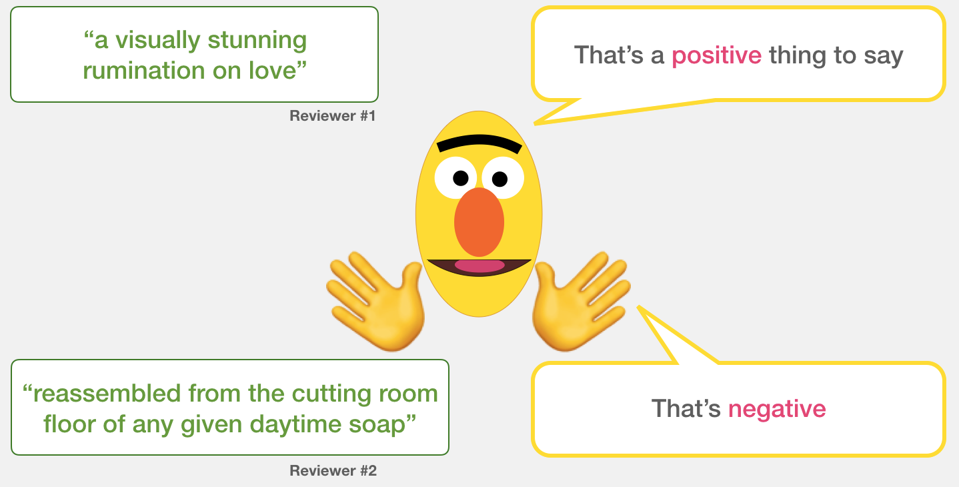
\includegraphics[width=\linewidth,keepaspectratio]{bert130}
			\end{center}	


\end{frame}

%%%%%%%%%%%%%%%%%%%%%%%%%%%%%%%%%%%%%%%%%%%%%%%%%%%%%%%%%%%
\begin{frame}[fragile]\frametitle{ SST2 Sentences from movie reviews}

			\begin{center}
			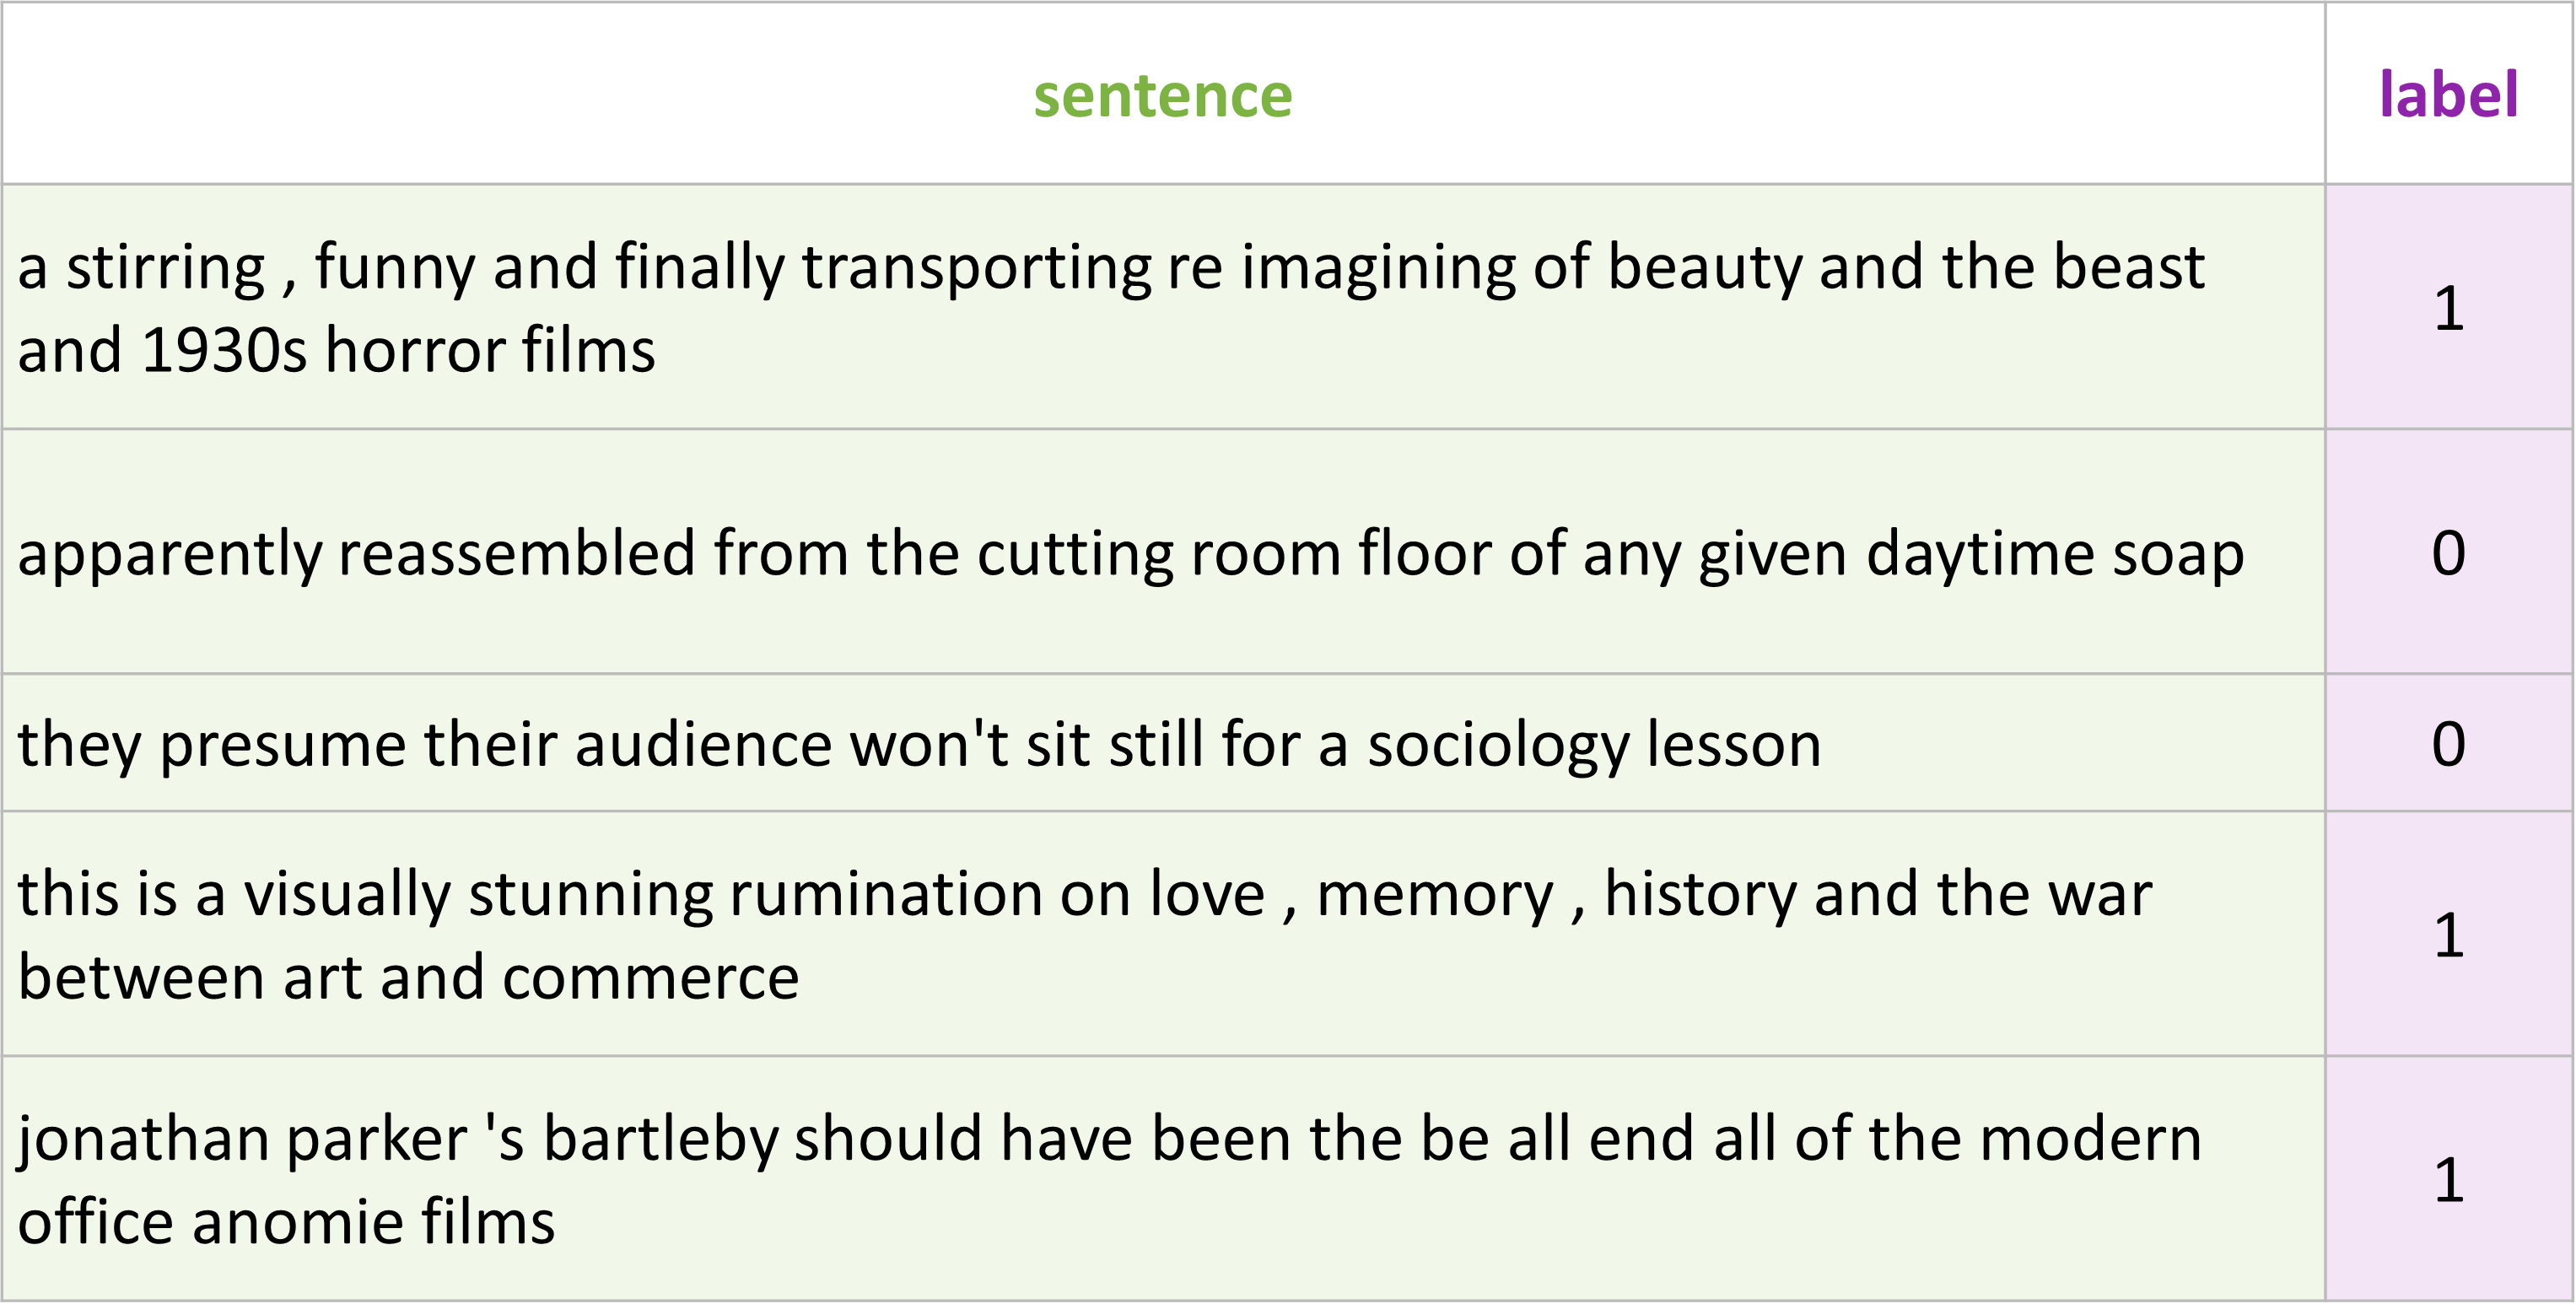
\includegraphics[width=\linewidth,keepaspectratio]{bert131}
			\end{center}	

% {\tiny (Ref: The Illustrated BERT, ELMo, and co. (How NLP Cracked Transfer Learning) – Jay Alammar)}

\end{frame}

%%%%%%%%%%%%%%%%%%%%%%%%%%%%%%%%%%%%%%%%%%%%%%%%%%%%%%%%%%%
\begin{frame}[fragile]\frametitle{ Movie Review Sentiment Classifier}

			\begin{center}
			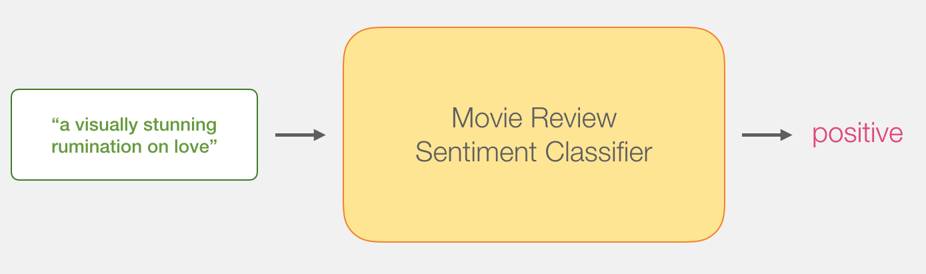
\includegraphics[width=\linewidth,keepaspectratio]{bert132}
			\end{center}	

% {\tiny (Ref: The Illustrated BERT, ELMo, and co. (How NLP Cracked Transfer Learning) – Jay Alammar)}

\end{frame}

%%%%%%%%%%%%%%%%%%%%%%%%%%%%%%%%%%%%%%%%%%%%%%%%%%%%%%%%%%%
\begin{frame}[fragile]\frametitle{ Movie Review Sentiment Classifier}

			\begin{center}
			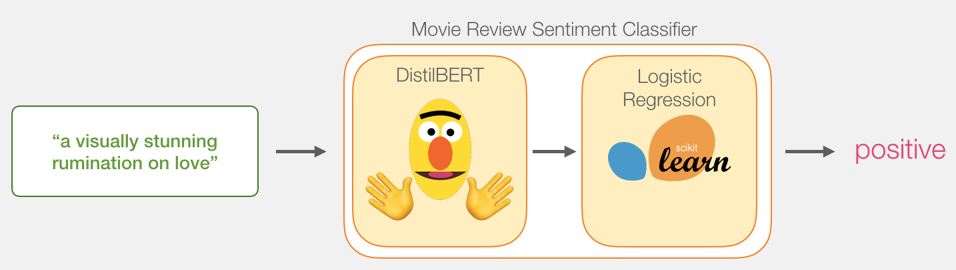
\includegraphics[width=\linewidth,keepaspectratio]{bert133}
			\end{center}	

% {\tiny (Ref: The Illustrated BERT, ELMo, and co. (How NLP Cracked Transfer Learning) – Jay Alammar)}

\end{frame}

%%%%%%%%%%%%%%%%%%%%%%%%%%%%%%%%%%%%%%%%%%%%%%%%%%%%%%%%%%%
\begin{frame}[fragile]\frametitle{ Movie Review Sentiment Classifier}

			\begin{center}
			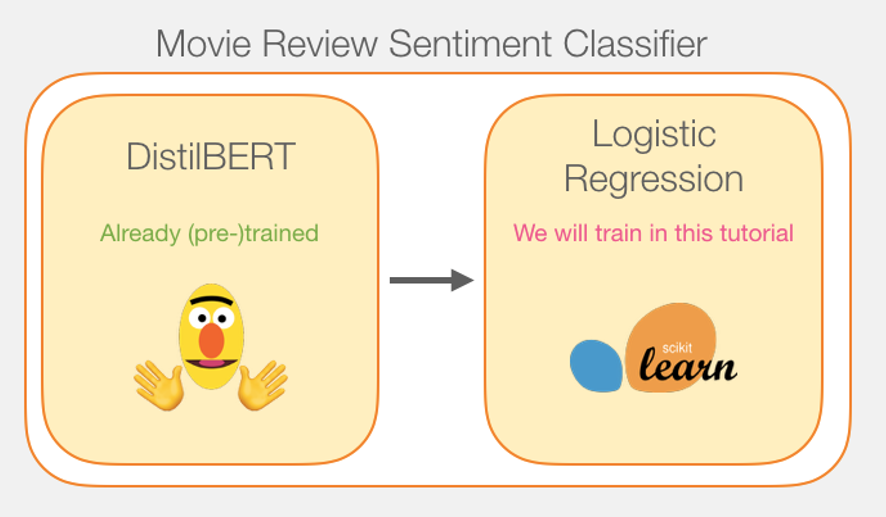
\includegraphics[width=\linewidth,keepaspectratio]{bert134}
			\end{center}	

% {\tiny (Ref: The Illustrated BERT, ELMo, and co. (How NLP Cracked Transfer Learning) – Jay Alammar)}

\end{frame}

%%%%%%%%%%%%%%%%%%%%%%%%%%%%%%%%%%%%%%%%%%%%%%%%%%%%%%%%%%%
\begin{frame}[fragile]\frametitle{ Step 1: Use distilBERT to Generate Sentence Embeddings}

			\begin{center}
			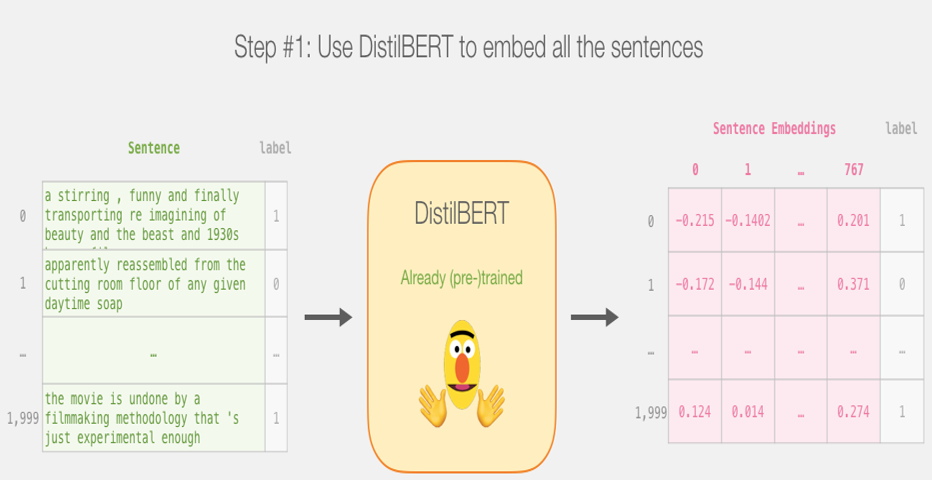
\includegraphics[width=\linewidth,keepaspectratio]{bert135}
			\end{center}	

% {\tiny (Ref: The Illustrated BERT, ELMo, and co. (How NLP Cracked Transfer Learning) – Jay Alammar)}

\end{frame}

%%%%%%%%%%%%%%%%%%%%%%%%%%%%%%%%%%%%%%%%%%%%%%%%%%%%%%%%%%%
\begin{frame}[fragile]\frametitle{ Step 2:Test/Train Split for Model 2, Logistic Regression}

			\begin{center}
			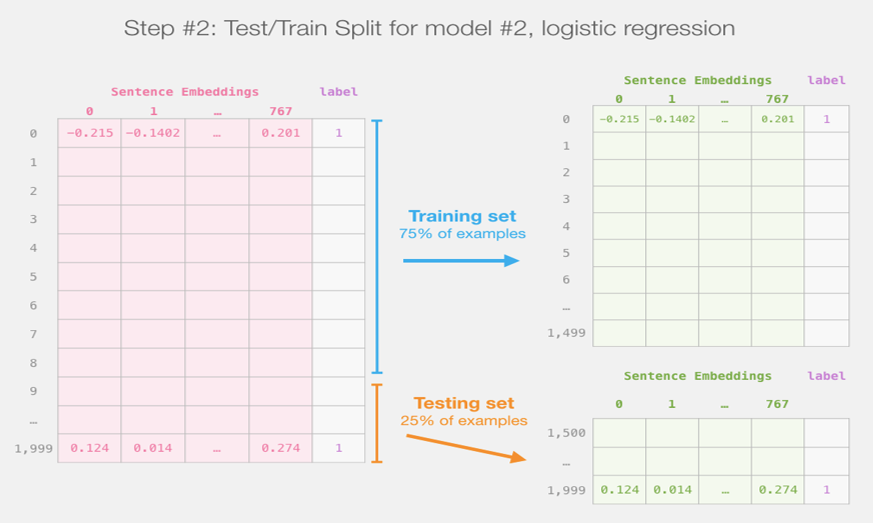
\includegraphics[width=\linewidth,keepaspectratio]{bert136}
			\end{center}	

% {\tiny (Ref: The Illustrated BERT, ELMo, and co. (How NLP Cracked Transfer Learning) – Jay Alammar)}

\end{frame}

%%%%%%%%%%%%%%%%%%%%%%%%%%%%%%%%%%%%%%%%%%%%%%%%%%%%%%%%%%%
\begin{frame}[fragile]\frametitle{ Step 3: Train the logistic regression model using the training set}

			\begin{center}
			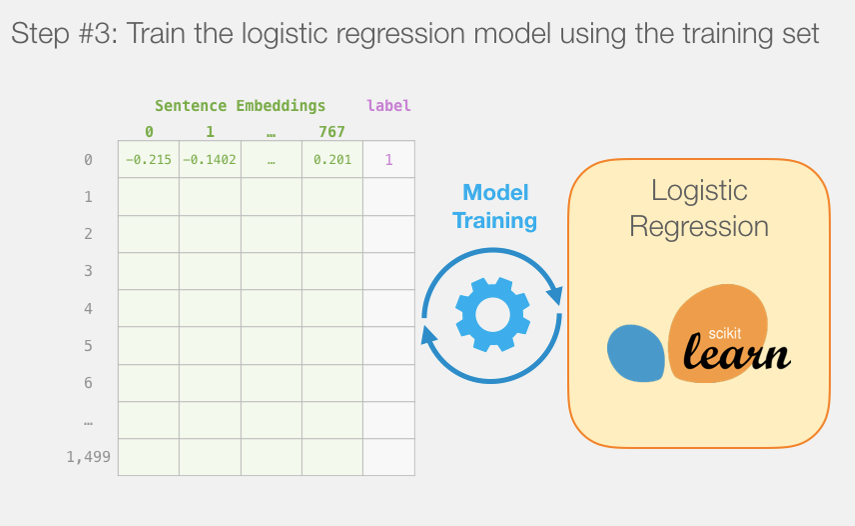
\includegraphics[width=\linewidth,keepaspectratio]{bert137}
			\end{center}	

% {\tiny (Ref: The Illustrated BERT, ELMo, and co. (How NLP Cracked Transfer Learning) – Jay Alammar)}

\end{frame}

%%%%%%%%%%%%%%%%%%%%%%%%%%%%%%%%%%%%%%%%%%%%%%%%%%%%%%%%%%%
\begin{frame}[fragile]\frametitle{ Tokenization}

[CLS] a visually stunning rum \#\#ination on love [SEP]
a visually stunning rumination on love


			\begin{center}
			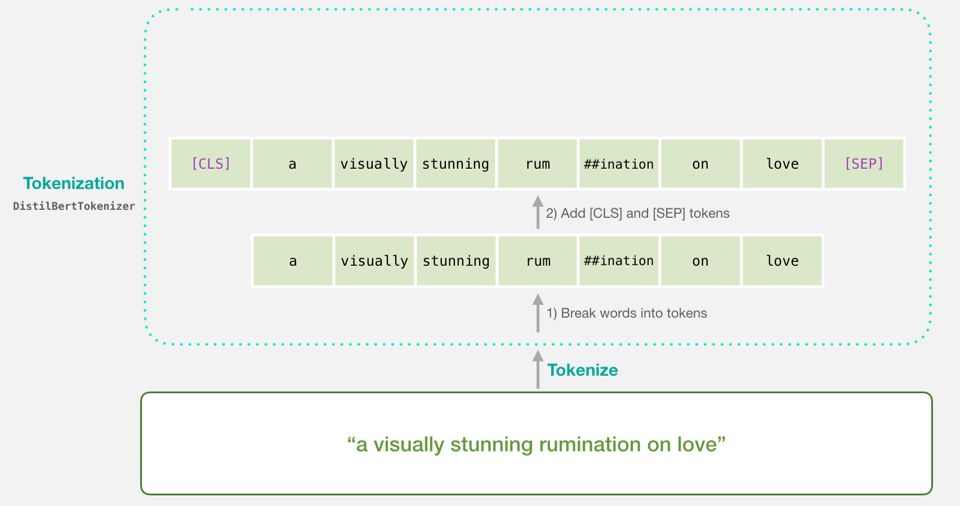
\includegraphics[width=\linewidth,keepaspectratio]{bert138}
			\end{center}	

% {\tiny (Ref: The Illustrated BERT, ELMo, and co. (How NLP Cracked Transfer Learning) – Jay Alammar)}

\end{frame}

%%%%%%%%%%%%%%%%%%%%%%%%%%%%%%%%%%%%%%%%%%%%%%%%%%%%%%%%%%%
\begin{frame}[fragile]\frametitle{ Tokenization}

\lstinline|tokenizer.encode("a visually stunning rumination on love", add_special_tokens=True)|


			\begin{center}
			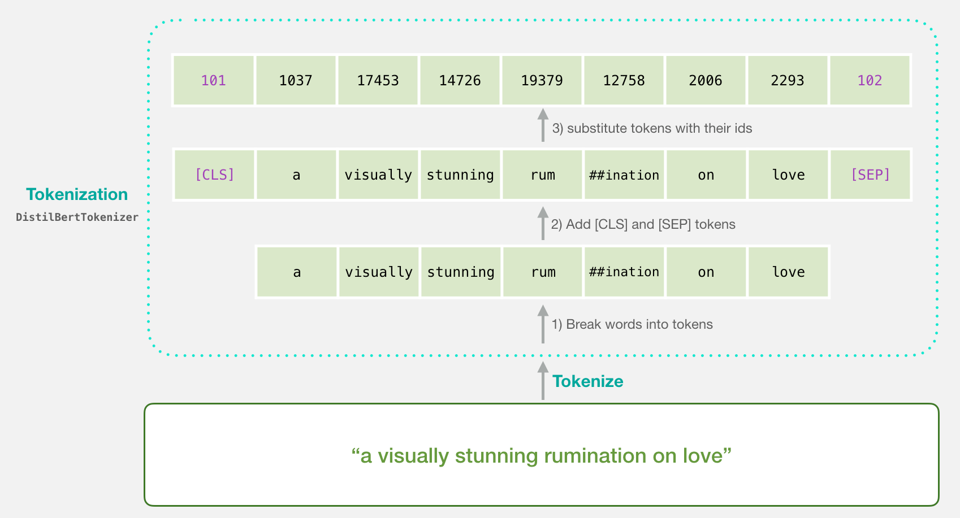
\includegraphics[width=\linewidth,keepaspectratio]{bert139}
			\end{center}	

% {\tiny (Ref: The Illustrated BERT, ELMo, and co. (How NLP Cracked Transfer Learning) – Jay Alammar)}

\end{frame}

%%%%%%%%%%%%%%%%%%%%%%%%%%%%%%%%%%%%%%%%%%%%%%%%%%%%%%%%%%%
\begin{frame}[fragile]\frametitle{ Tokenization for BERT Model}

			\begin{center}
			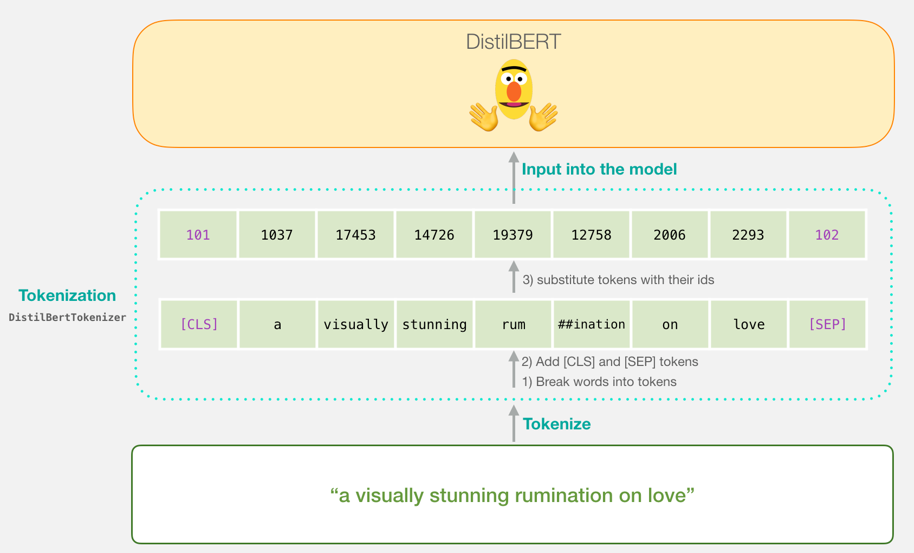
\includegraphics[width=\linewidth,keepaspectratio]{bert140}
			\end{center}	

% {\tiny (Ref: The Illustrated BERT, ELMo, and co. (How NLP Cracked Transfer Learning) – Jay Alammar)}

\end{frame}

%%%%%%%%%%%%%%%%%%%%%%%%%%%%%%%%%%%%%%%%%%%%%%%%%%%%%%%%%%%
\begin{frame}[fragile]\frametitle{ Flowing Through DistilBERT (768 features)}

			\begin{center}
			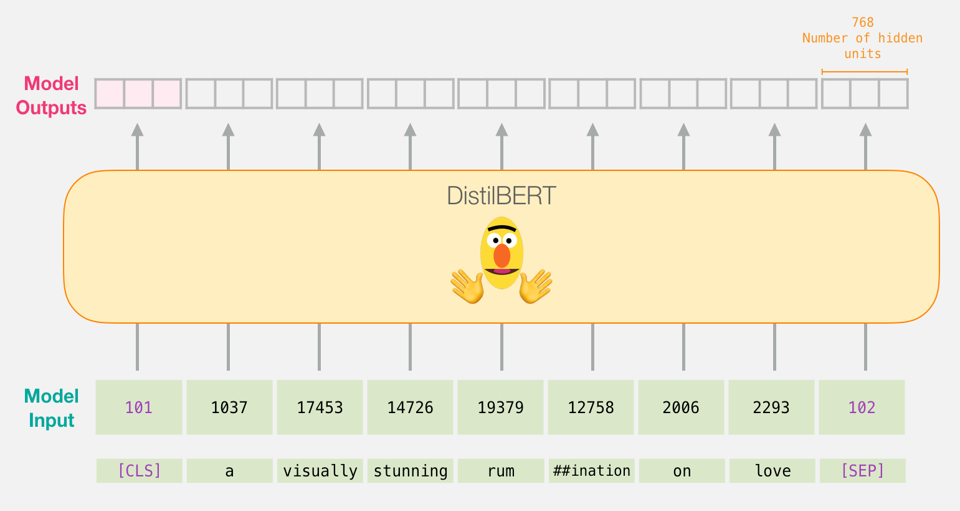
\includegraphics[width=\linewidth,keepaspectratio]{bert141}
			\end{center}	

% {\tiny (Ref: The Illustrated BERT, ELMo, and co. (How NLP Cracked Transfer Learning) – Jay Alammar)}

\end{frame}

%%%%%%%%%%%%%%%%%%%%%%%%%%%%%%%%%%%%%%%%%%%%%%%%%%%%%%%%%%%
\begin{frame}[fragile]\frametitle{ Model 1 Output Class vector as Model 2 Input}

			\begin{center}
			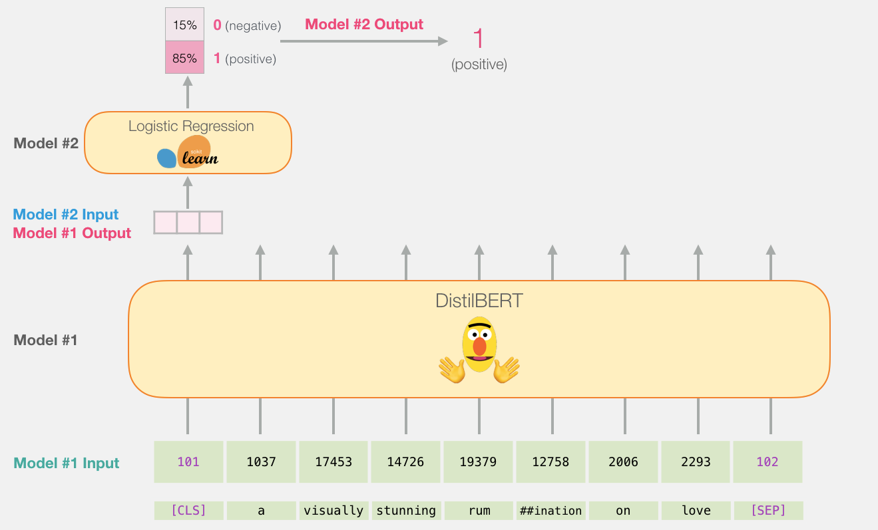
\includegraphics[width=\linewidth,keepaspectratio]{bert142}
			\end{center}	

% {\tiny (Ref: The Illustrated BERT, ELMo, and co. (How NLP Cracked Transfer Learning) – Jay Alammar)}

\end{frame}

%%%%%%%%%%%%%%%%%%%%%%%%%%%%%%%%%%%%%%%%%%%%%%%%%%%%%%%%%%%
\begin{frame}[fragile]\frametitle{ Fine-tuning BERT on Single Sentence Classification Tasks}

			\begin{center}
			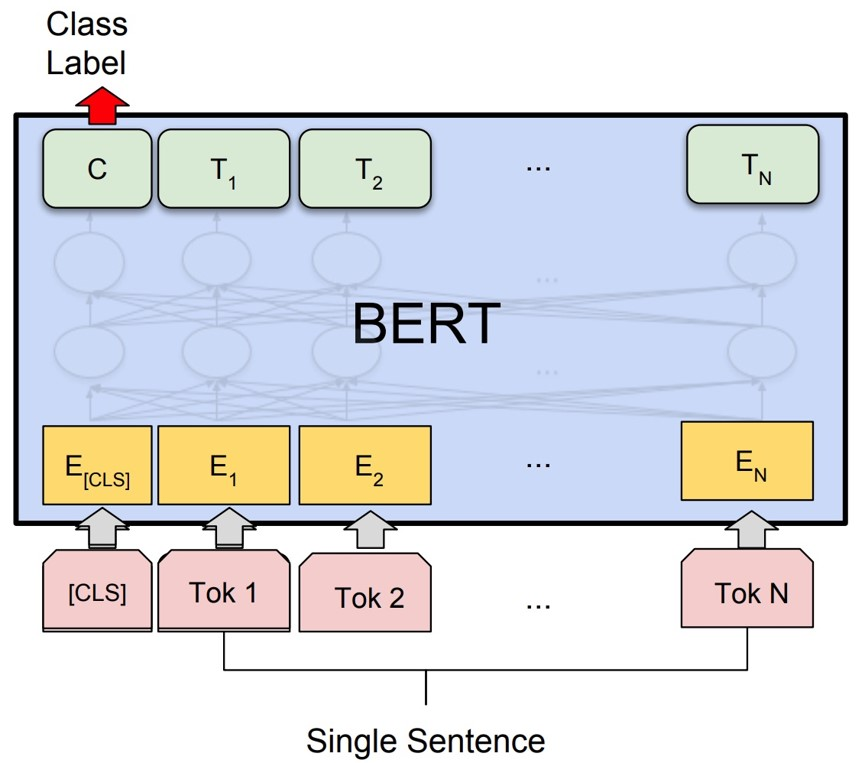
\includegraphics[width=0.5\linewidth,keepaspectratio]{bert143}
			\end{center}	

% {\tiny (Ref: The Illustrated BERT, ELMo, and co. (How NLP Cracked Transfer Learning) – Jay Alammar)}

\end{frame}

%%%%%%%%%%%%%%%%%%%%%%%%%%%%%%%%%%%%%%%%%%%%%%%%%%%%%%%%%%%
\begin{frame}[fragile]\frametitle{ Model 1 Output Class vector as Model 2 Input}

			\begin{center}
			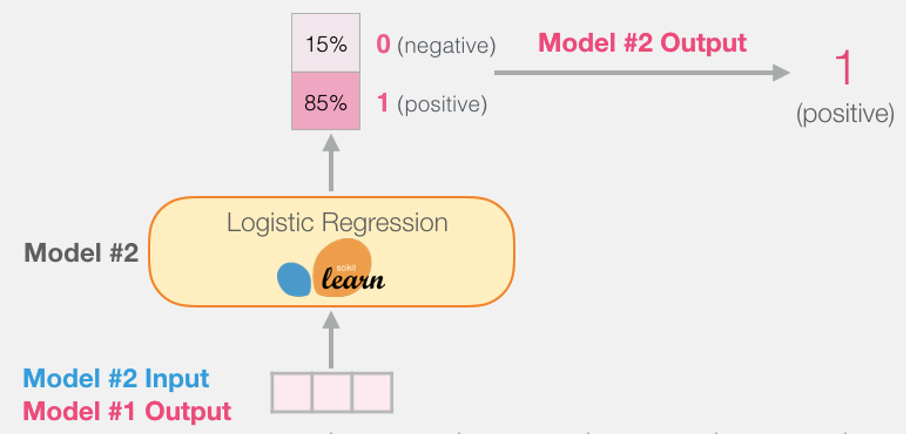
\includegraphics[width=\linewidth,keepaspectratio]{bert144}
			\end{center}	

% {\tiny (Ref: The Illustrated BERT, ELMo, and co. (How NLP Cracked Transfer Learning) – Jay Alammar)}

\end{frame}

%%%%%%%%%%%%%%%%%%%%%%%%%%%%%%%%%%%%%%%%%%%%%%%%%%%%%%%%%%%
\begin{frame}[fragile]\frametitle{ Logistic Regression Model to classify Class vector }

			\begin{center}
			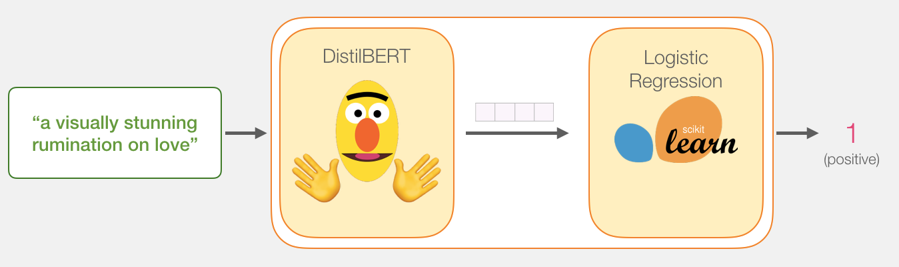
\includegraphics[width=\linewidth,keepaspectratio]{bert145}
			\end{center}	

% {\tiny (Ref: The Illustrated BERT, ELMo, and co. (How NLP Cracked Transfer Learning) – Jay Alammar)}

\end{frame}

%%%%%%%%%%%%%%%%%%%%%%%%%%%%%%%%%%%%%%%%%%%%%%%%%%%%%%%%%%%
\begin{frame}[fragile]\frametitle{Inputs}



			\begin{center}
			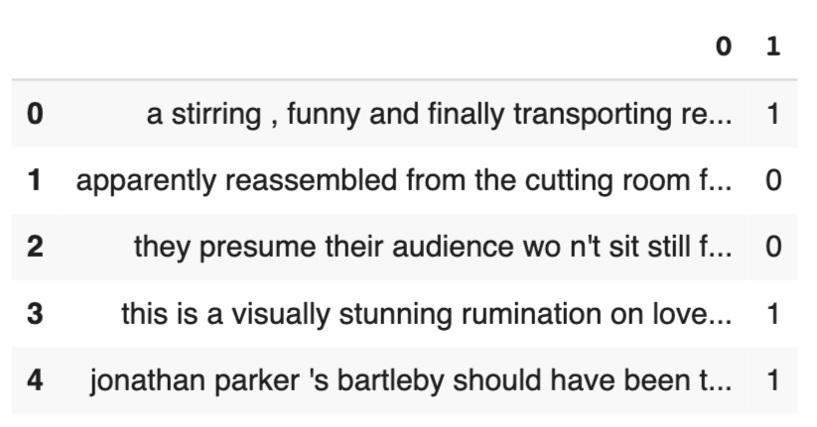
\includegraphics[width=0.8\linewidth,keepaspectratio]{bert146}
			\end{center}	

\begin{lstlisting}
df = pd.read_csv('https://github.com/clairett/pytorch-sentiment-classification/raw/master/data/SST2/train.tsv', delimiter='\t', header=None)

df.head()
\end{lstlisting}

% % {\tiny (Ref: The Illustrated BERT, ELMo, and co. (How NLP Cracked Transfer Learning) – Jay Alammar)}

\end{frame}

%%%%%%%%%%%%%%%%%%%%%%%%%%%%%%%%%%%%%%%%%%%%%%%%%%%%%%%%%%%
\begin{frame}[fragile]\frametitle{Tokenization}

% \begin{lstlisting}
% tokenized = df[0].apply((lambda x: tokenizer.encode(x, add_special_tokens=True)))
% \end{lstlisting}

			\begin{center}
			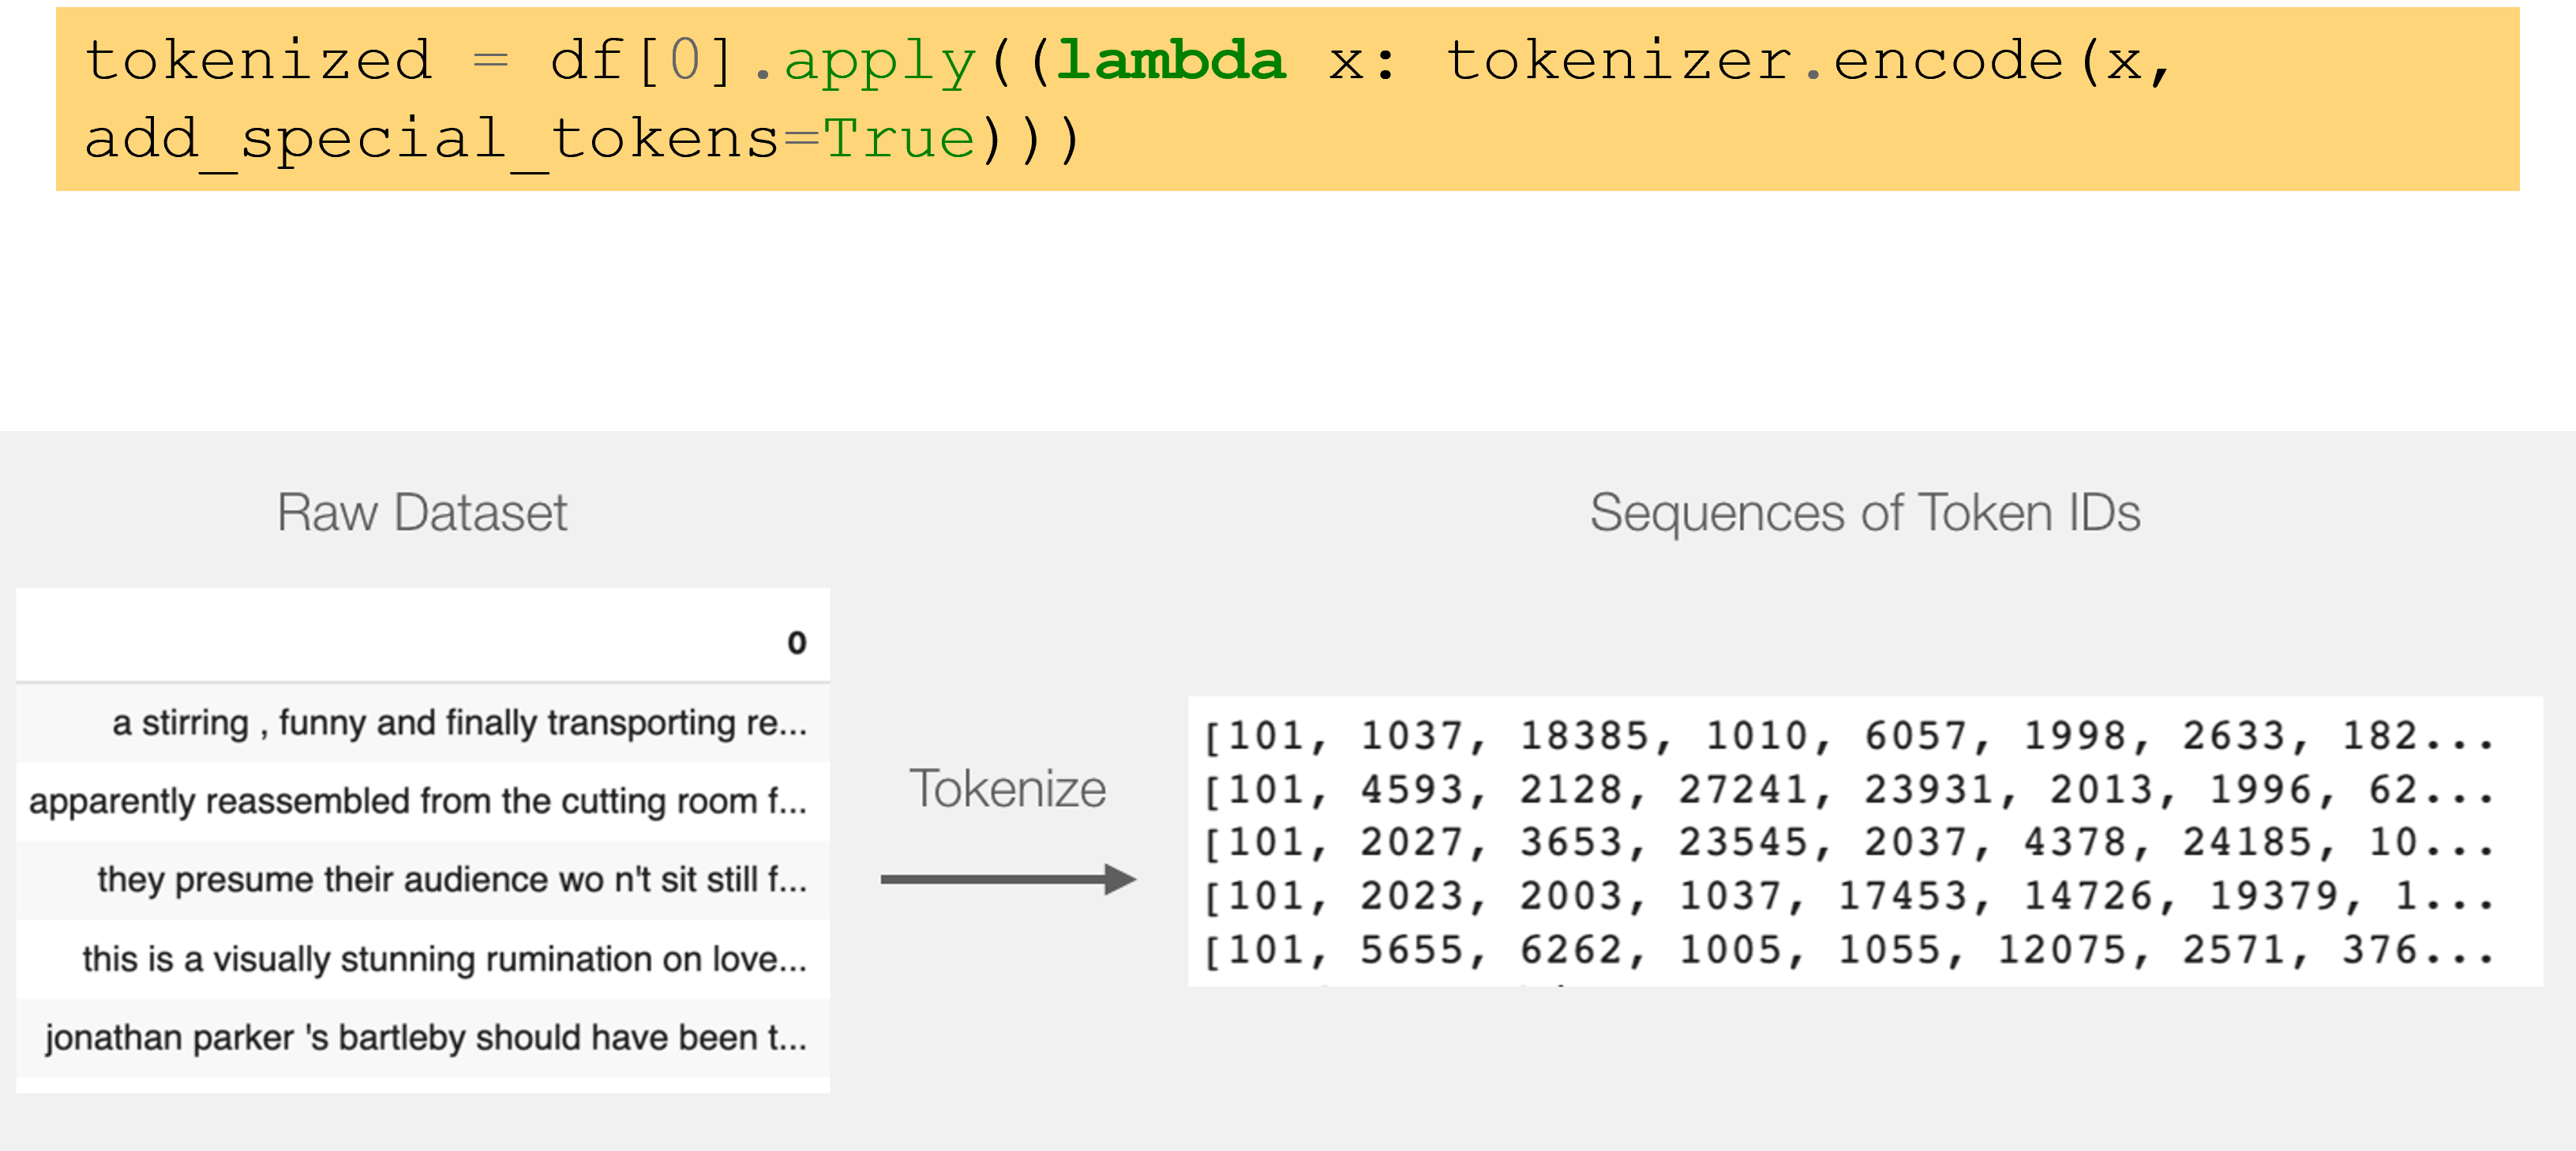
\includegraphics[width=\linewidth,keepaspectratio]{bert147}
			\end{center}	

% {\tiny (Ref: The Illustrated BERT, ELMo, and co. (How NLP Cracked Transfer Learning) – Jay Alammar)}

\end{frame}

%%%%%%%%%%%%%%%%%%%%%%%%%%%%%%%%%%%%%%%%%%%%%%%%%%%%%%%%%%%
\begin{frame}[fragile]\frametitle{BERT Input Tensor}

			\begin{center}
			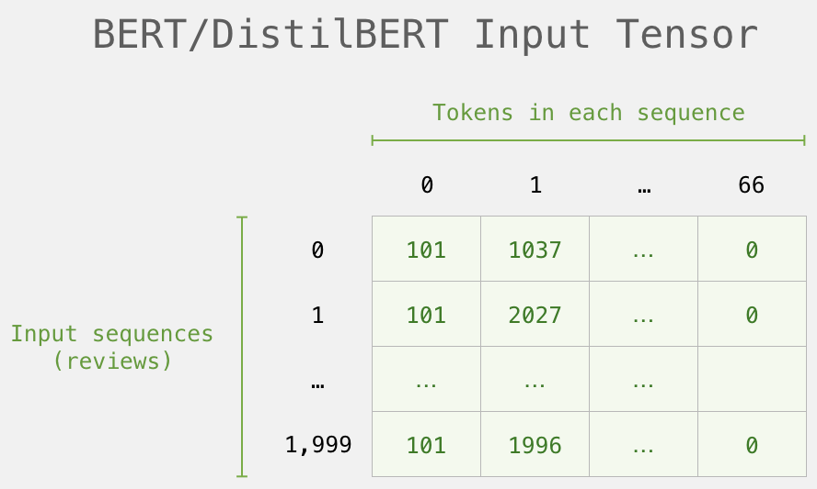
\includegraphics[width=\linewidth,keepaspectratio]{bert148}
			\end{center}	

% {\tiny (Ref: The Illustrated BERT, ELMo, and co. (How NLP Cracked Transfer Learning) – Jay Alammar)}

\end{frame}

%%%%%%%%%%%%%%%%%%%%%%%%%%%%%%%%%%%%%%%%%%%%%%%%%%%%%%%%%%%
\begin{frame}[fragile]\frametitle{Processing with DistilBERT}



			\begin{center}
			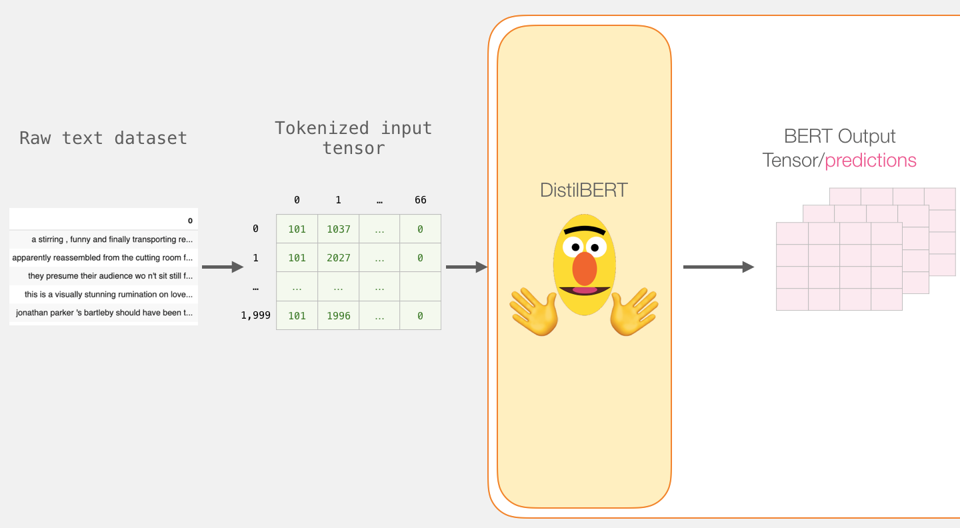
\includegraphics[width=\linewidth,keepaspectratio]{bert149}
			\end{center}	

\begin{lstlisting}
input_ids = torch.tensor(np.array(padded))
last_hidden_states = model(input_ids)
\end{lstlisting}


% % {\tiny (Ref: The Illustrated BERT, ELMo, and co. (How NLP Cracked Transfer Learning) – Jay Alammar)}

\end{frame}

%%%%%%%%%%%%%%%%%%%%%%%%%%%%%%%%%%%%%%%%%%%%%%%%%%%%%%%%%%%
\begin{frame}[fragile]\frametitle{Unpacking the BERT output tensor}

			\begin{center}
			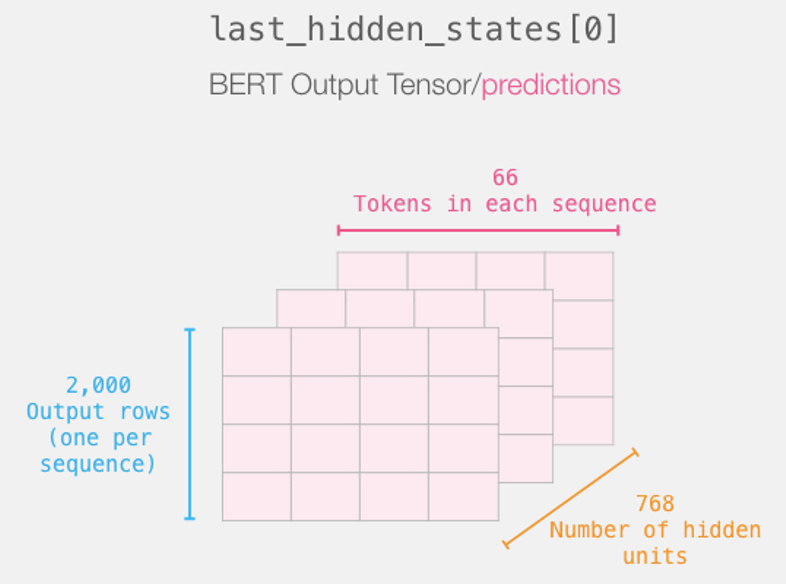
\includegraphics[width=0.8\linewidth,keepaspectratio]{bert150}
			\end{center}	

% {\tiny (Ref: The Illustrated BERT, ELMo, and co. (How NLP Cracked Transfer Learning) – Jay Alammar)}

\end{frame}

%%%%%%%%%%%%%%%%%%%%%%%%%%%%%%%%%%%%%%%%%%%%%%%%%%%%%%%%%%%
\begin{frame}[fragile]\frametitle{Sentence to last\_hidden\_state[0]}

			\begin{center}
			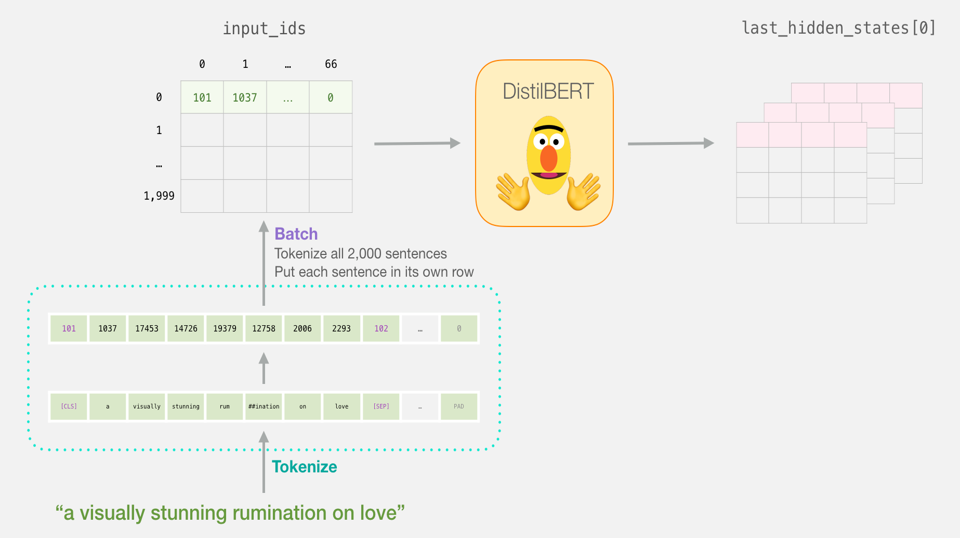
\includegraphics[width=\linewidth,keepaspectratio]{bert151}
			\end{center}	

% {\tiny (Ref: The Illustrated BERT, ELMo, and co. (How NLP Cracked Transfer Learning) – Jay Alammar)}

\end{frame}


%%%%%%%%%%%%%%%%%%%%%%%%%%%%%%%%%%%%%%%%%%%%%%%%%%%%%%%%%%%
\begin{frame}[fragile]\frametitle{BERT’s output for the [CLS] tokens}



			\begin{center}
			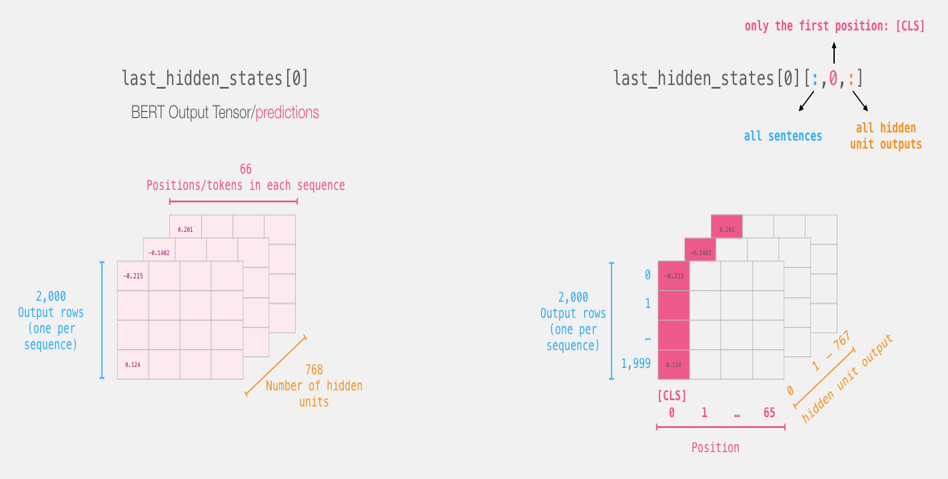
\includegraphics[width=\linewidth,keepaspectratio]{bert152}
			\end{center}	

\begin{lstlisting}
# Slice the output for the first position for all the sequences, take all hidden unit outputs 
features = last_hidden_states[0][:,0,:].numpy()
\end{lstlisting}


% % {\tiny (Ref: The Illustrated BERT, ELMo, and co. (How NLP Cracked Transfer Learning) – Jay Alammar)}

\end{frame}


%%%%%%%%%%%%%%%%%%%%%%%%%%%%%%%%%%%%%%%%%%%%%%%%%%%%%%%%%%%
\begin{frame}[fragile]\frametitle{The tensor sliced from BERT's output Sentence Embeddings}


			\begin{center}
			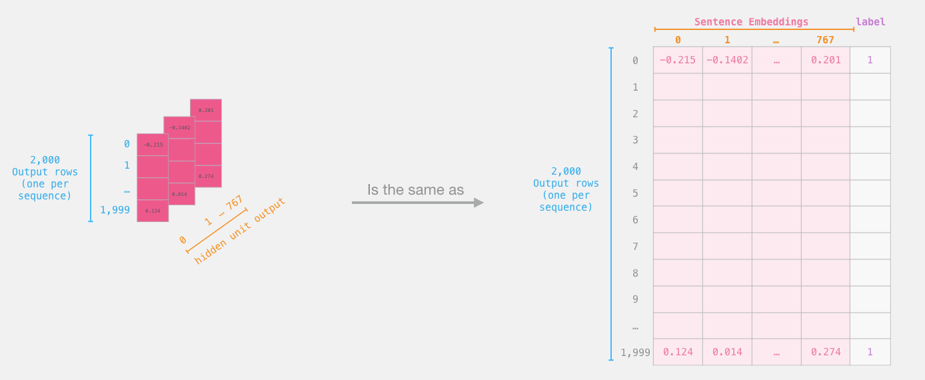
\includegraphics[width=\linewidth,keepaspectratio]{bert153}
			\end{center}	

% {\tiny (Ref: The Illustrated BERT, ELMo, and co. (How NLP Cracked Transfer Learning) – Jay Alammar)}

\end{frame}

%%%%%%%%%%%%%%%%%%%%%%%%%%%%%%%%%%%%%%%%%%%%%%%%%%%%%%%%%%%
\begin{frame}[fragile]\frametitle{Dataset for Logistic Regression (768 Features)}

The features are the output vectors of BERT for the [CLS] token (position \#0)

			\begin{center}
			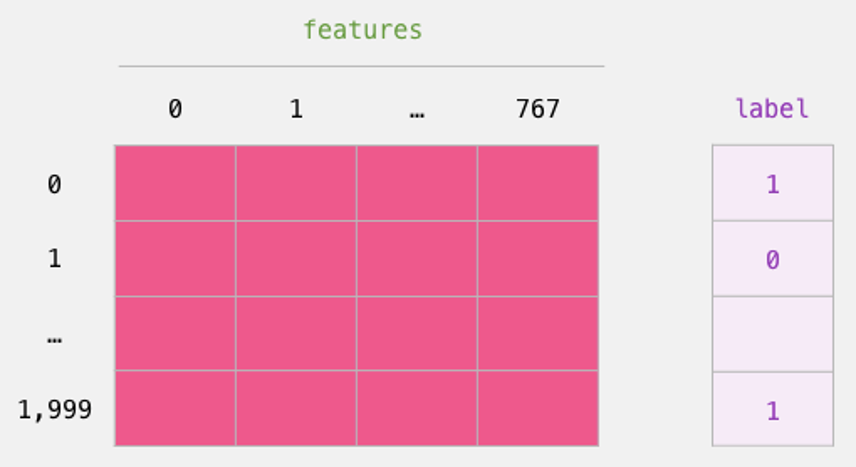
\includegraphics[width=\linewidth,keepaspectratio]{bert154}
			\end{center}	

% {\tiny (Ref: The Illustrated BERT, ELMo, and co. (How NLP Cracked Transfer Learning) – Jay Alammar)}

\end{frame}

%%%%%%%%%%%%%%%%%%%%%%%%%%%%%%%%%%%%%%%%%%%%%%%%%%%%%%%%%%%
\begin{frame}[fragile]\frametitle{}

			\begin{center}
			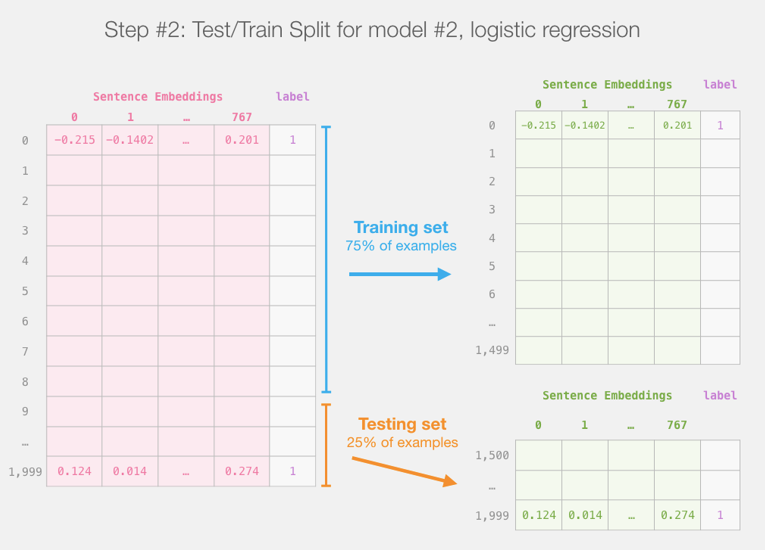
\includegraphics[width=\linewidth,keepaspectratio]{bert155}
			\end{center}	
			
\begin{lstlisting}
labels = df[1]
train_features, test_features, train_labels, test_labels = train_test_split(features, labels)
\end{lstlisting}




% {\tiny (Ref: The Illustrated BERT, ELMo, and co. (How NLP Cracked Transfer Learning) – Jay Alammar)}

\end{frame}

%%%%%%%%%%%%%%%%%%%%%%%%%%%%%%%%%%%%%%%%%%%%%%%%%%%%%%%%%%%
\begin{frame}[fragile]\frametitle{Score Benchmarks Logistic Regression Model on SST-2 Dataset }

\begin{lstlisting}
# Training
lr_clf = LogisticRegression() 
lr_clf.fit(train_features, train_labels)

#Testing
lr_clf.score(test_features, test_labels)

# Accuracy: 81%
# Highest accuracy: 96.8%
# Fine-tuned DistilBERT: 90.7%
# Full size BERT model: 94.9%
\end{lstlisting}


% % {\tiny (Ref: The Illustrated BERT, ELMo, and co. (How NLP Cracked Transfer Learning) – Jay Alammar)}

\end{frame}

% %%%%%%%%%%%%%%%%%%%%%%%%%%%%%%%%%%%%%%%%%%%%%%%%%%%%%%%%%%%
% \begin{frame}[fragile]\frametitle{Sentiment Classification: SST2 Sentences from movie reviews}

			% \begin{center}
			% 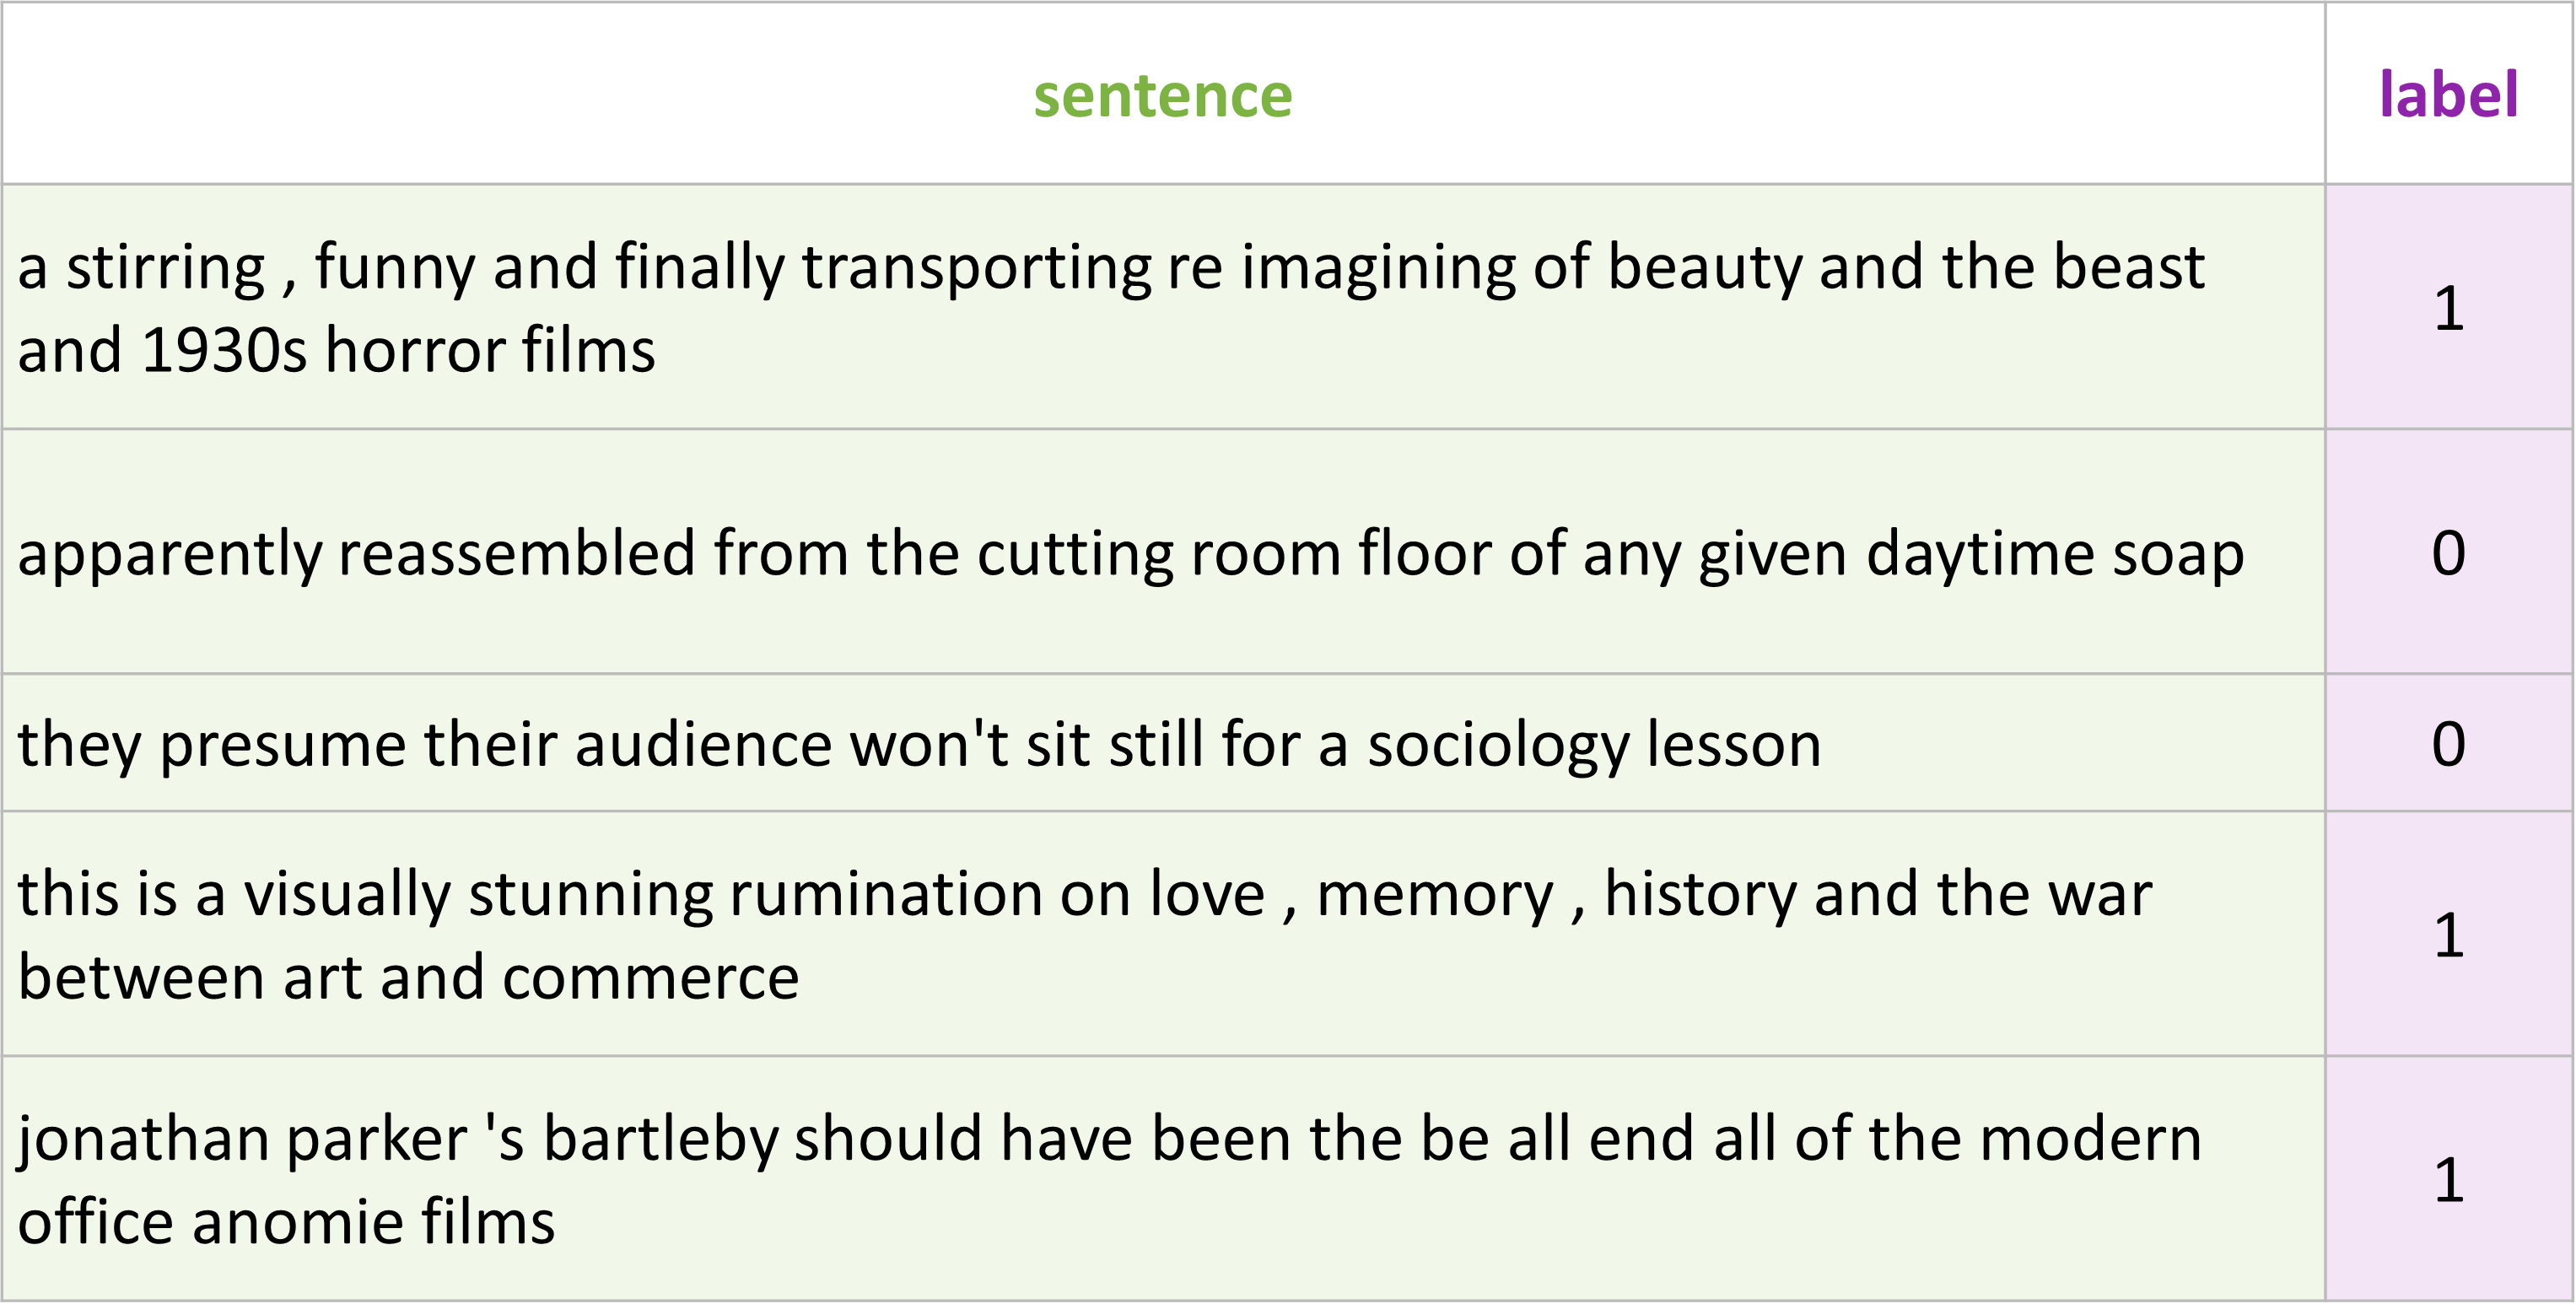
\includegraphics[width=\linewidth,keepaspectratio]{bert156}
			% \end{center}	

% % {\tiny (Ref: The Illustrated BERT, ELMo, and co. (How NLP Cracked Transfer Learning) – Jay Alammar)}

% \end{frame}

% %%%%%%%%%%%%%%%%%%%%%%%%%%%%%%%%%%%%%%%%%%%%%%%%%%%%%%%%%%%
% \begin{frame}[fragile]\frametitle{A Visual Notebook to Using BERT for the First Time }

			% \begin{center}
			% 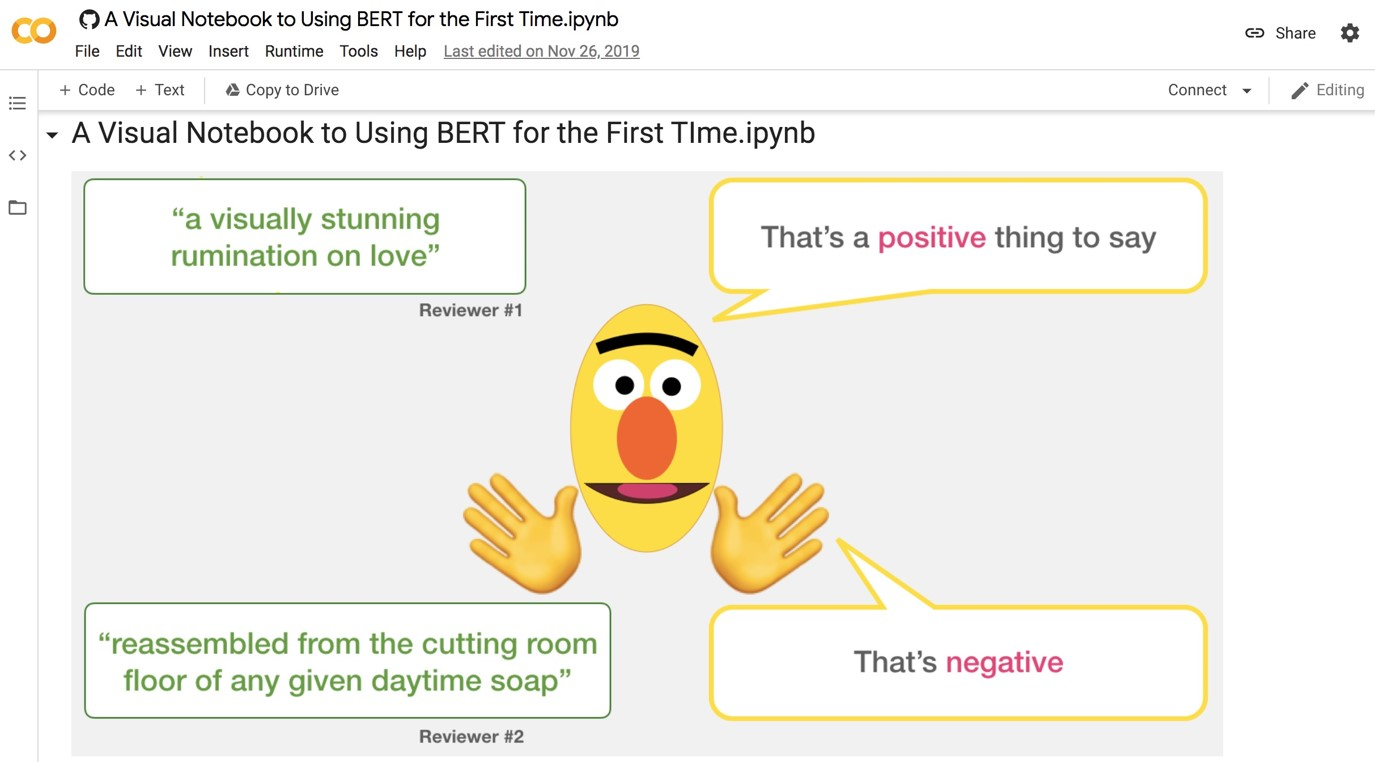
\includegraphics[width=\linewidth,keepaspectratio]{bert157}
			% \end{center}	

% % {\tiny (Ref: The Illustrated BERT, ELMo, and co. (How NLP Cracked Transfer Learning) – Jay Alammar)}

% \end{frame}

%%%%%%%%%%%%%%%%%%%%%%%%%%%%%%%%%%%%%%%%%%%%%%%%%%%%%%%%%%%%%%%%%%%%%%%%%%%%%%%%%
% \begin{frame}[fragile]\frametitle{}
% \begin{center}
% {\Large BERT Variants}
% \end{center}
% \end{frame}
